\section{Supplementary material}


\subsection{Descriptive statistics}

\small
\renewcommand{\arraystretch}{1.3}
\begin{longtable}{p{7cm} p{1cm} p{0.8cm} p{0.8cm} p{0.8cm} p{0.8cm} p{0.8cm} p{0.8cm} p{0.8cm} p{0.8cm}}
\caption{Descriptive statistics for all patients arriving at each stroke team. The table shows summary statistics across all stroke teams.}\\
\toprule
\endhead
Statistic & Stroke teams & mean & Std Dev & min & 25\% & 50\% & 75\% & max\tabularnewline
\midrule
Yearly admissions & 117 & 516 & 203 & 139 & 380 & 491 & 627 & 1183\tabularnewline
Age (mean) & 117 & 74 & 2 & 65 & 73 & 75 & 76 & 78\tabularnewline
Proportion aged 80+ & 117 & 0.40 & 0.06 & 0.20 & 0.36 & 0.40 & 0.44 & 0.51\tabularnewline
Proportion male & 117 & 0.53 & 0.02 & 0.47 & 0.51 & 0.53 & 0.55 & 0.60\tabularnewline
Prior disability (mRS, mean) & 117 & 1.03 & 0.24 & 0.39 & 0.87 & 1.03 & 1.21 & 1.60\tabularnewline
Proportion prior disability (mRS) 0-2 & 117 & 0.81 & 0.05 & 0.67 & 0.78 & 0.81 & 0.84 & 0.95\tabularnewline
Proportion ischaemic stroke & 117 & 0.88 & 0.02 & 0.83 & 0.86 & 0.88 & 0.89 & 0.93\tabularnewline
Stroke severity (NIHSS, mean) & 117 & 7.06 & 0.95 & 4.59 & 6.32 & 7.23 & 7.79 & 9.06\tabularnewline
Proportion with known onset & 117 & 0.68 & 0.14 & 0.43 & 0.58 & 0.67 & 0.76 & 1.00\tabularnewline
Onset-to-arrival time (minutes, median) & 117 & 203 & 76 & 109 & 154 & 177 & 222 & 466\tabularnewline
Proportion arriving within 4 hours known onset & 117 & 0.38 & 0.06 & 0.19 & 0.34 & 0.38 & 0.42 & 0.51\tabularnewline
Proportion with precisely known onset & 117 & 0.33 & 0.11 & 0.01 & 0.28 & 0.34 & 0.39 & 0.63\tabularnewline
Proportion onset during sleep & 117 & 0.14 & 0.06 & 0.00 & 0.09 & 0.14 & 0.17 & 0.34\tabularnewline
Proportion arrive by ambulance & 117 & 0.78 & 0.07 & 0.53 & 0.76 & 0.79 & 0.82 & 0.92\tabularnewline
Call-to-ambulance arrival time (minutes, median) & 111 & 21 & 6 & 13 & 17 & 20 & 23 & 51\tabularnewline
Ambulance on scene time (median) & 111 & 31 & 3 & 20 & 28 & 31 & 33 & 41\tabularnewline
Ambulance conveyance time (minutes, median) & 111 & 18 & 5 & 10 & 15 & 17 & 21 & 37\tabularnewline
Arrival-to-scan time (minutes, median) & 117 & 53 & 21 & 13 & 39 & 52 & 64 & 129\tabularnewline
Proportion receiving thrombolysis & 117 & 0.114 & 0.033 & 0.021 & 0.091 & 0.109 & 0.136 & 0.245\tabularnewline
Scan-to-thrombolysis time (minutes, median) & 117 & 34 & 10 & 14 & 28 & 34 & 40 & 72\tabularnewline
Discharge disability (mRS, mean) & 117 & 2.65 & 0.33 & 1.65 & 2.42 & 2.70 & 2.90 & 3.32\tabularnewline
Proportion discharged mRS 0-2 & 117 & 0.52 & 0.09 & 0.29 & 0.46 & 0.52 & 0.59 & 0.72\tabularnewline
Proportion discharged mRS 5-6 & 117 & 0.20 & 0.04 & 0.10 & 0.17 & 0.20 & 0.22 & 0.29\tabularnewline
\bottomrule
\label{tab:hospital_stats_1}
\end{longtable}
\normalsize

\small
\begin{longtable}{p{7cm} p{1cm} p{0.8cm} p{0.8cm} p{0.8cm} p{0.8cm} p{0.8cm} p{0.8cm} p{0.8cm} p{0.8cm}}
\caption{Descriptive statistics for patients arriving at each stroke team, for patients arriving within 4 hours of known stroke onset. The table shows summary statistics across all stroke teams.}\\
\toprule
\endhead
Statistic & Stroke teams & mean & Std Dev & min & 25\% & 50\% & 75\% & max\tabularnewline
\midrule
Yearly admissions & 117 & 195 & 76 & 32 & 146 & 187 & 244 & 428\tabularnewline
Age (mean) & 117 & 75 & 2 & 66 & 73 & 75 & 76 & 79\tabularnewline
Proportion aged 80+ & 117 & 0.41 & 0.06 & 0.23 & 0.37 & 0.41 & 0.45 & 0.57\tabularnewline
Proportion male & 117 & 0.53 & 0.03 & 0.45 & 0.51 & 0.53 & 0.55 & 0.60\tabularnewline
Prior disability (mRS, mean) & 117 & 1.05 & 0.24 & 0.42 & 0.89 & 1.04 & 1.23 & 1.60\tabularnewline
Proportion prior disability (mRS) 0-2 & 117 & 0.80 & 0.05 & 0.66 & 0.77 & 0.80 & 0.83 & 0.94\tabularnewline
Proportion ischaemic stroke & 117 & 0.85 & 0.03 & 0.75 & 0.84 & 0.85 & 0.87 & 0.94\tabularnewline
Stroke severity (NIHSS, mean) & 117 & 8.95 & 1.04 & 6.44 & 8.21 & 9.00 & 9.68 & 11.43\tabularnewline
Proportion with known onset & 117 & 1.00 & 0.00 & 1.00 & 1.00 & 1.00 & 1.00 & 1.00\tabularnewline
Onset-to-arrival time (minutes, median) & 117 & 105 & 9 & 85 & 100 & 105 & 110 & 126\tabularnewline
Proportion arriving within 4 hours known onset & 117 & 1.00 & 0.00 & 1.00 & 1.00 & 1.00 & 1.00 & 1.00\tabularnewline
Proportion with precisely known onset & 117 & 0.62 & 0.18 & 0.02 & 0.52 & 0.66 & 0.75 & 0.91\tabularnewline
Proportion onset during sleep & 117 & 0.05 & 0.05 & 0.00 & 0.01 & 0.03 & 0.06 & 0.30\tabularnewline
Proportion arrive by ambulance & 117 & 0.90 & 0.06 & 0.65 & 0.88 & 0.91 & 0.93 & 0.98\tabularnewline
Call-to-ambulance arrival time (minutes, median) & 109 & 19 & 5 & 8 & 16 & 18 & 21 & 51\tabularnewline
Ambulance on scene time (median) & 109 & 28 & 3 & 20 & 26 & 28 & 31 & 41\tabularnewline
Ambulance conveyance time (minutes, median) & 109 & 17 & 4 & 9 & 14 & 16 & 20 & 28\tabularnewline
Arrival-to-scan time (minutes, median) & 117 & 28 & 11 & 4 & 21 & 28 & 34 & 100\tabularnewline
Proportion receiving thrombolysis & 117 & 0.290 & 0.067 & 0.111 & 0.249 & 0.281 & 0.327 & 0.479\tabularnewline
Scan-to-thrombolysis time (minutes, median) & 117 & 34 & 10 & 14 & 27 & 34 & 40 & 71\tabularnewline
Discharge disability (mRS, mean) & 117 & 2.81 & 0.33 & 1.80 & 2.61 & 2.84 & 3.04 & 3.66\tabularnewline
Proportion discharged mRS 0-2 & 117 & 0.49 & 0.09 & 0.21 & 0.42 & 0.50 & 0.55 & 0.71\tabularnewline
Proportion discharged mRS 5-6 & 117 & 0.24 & 0.04 & 0.14 & 0.21 & 0.23 & 0.26 & 0.42\tabularnewline
\bottomrule
\label{tab:hospital_stats_2}
\end{longtable}
\normalsize

\small
\begin{longtable}{p{7cm} p{1cm} p{0.8cm} p{0.8cm} p{0.8cm} p{0.8cm} p{0.8cm} p{0.8cm} p{0.8cm} p{0.8cm}}
\caption{Descriptive statistics for patients arriving at each stroke team, for patients arriving by ambulance within 4 hours of known stroke onset. The table shows summary statistics across all stroke teams.}\\
\toprule
\endhead
Statistic & Stroke teams & mean & Std Dev & min & 25\% & 50\% & 75\% & max\tabularnewline
\midrule
Yearly admissions & 117 & 176 & 72 & 28 & 126 & 164 & 228 & 400\tabularnewline
Age (mean) & 117 & 75 & 2 & 66 & 74 & 76 & 77 & 81\tabularnewline
Proportion aged 80+ & 117 & 0.43 & 0.06 & 0.24 & 0.39 & 0.43 & 0.47 & 0.62\tabularnewline
Proportion male & 117 & 0.52 & 0.03 & 0.45 & 0.51 & 0.52 & 0.54 & 0.60\tabularnewline
Prior disability (mRS, mean) & 117 & 1.10 & 0.25 & 0.46 & 0.94 & 1.09 & 1.26 & 1.66\tabularnewline
Proportion prior disability (mRS) 0-2 & 117 & 0.79 & 0.06 & 0.65 & 0.75 & 0.79 & 0.82 & 0.93\tabularnewline
Proportion ischaemic stroke & 117 & 0.85 & 0.03 & 0.75 & 0.83 & 0.85 & 0.87 & 0.94\tabularnewline
Stroke severity (NIHSS, mean) & 117 & 9.41 & 1.18 & 6.72 & 8.55 & 9.45 & 10.20 & 12.23\tabularnewline
Proportion with known onset & 117 & 1.00 & 0.00 & 1.00 & 1.00 & 1.00 & 1.00 & 1.00\tabularnewline
Onset-to-arrival time (minutes, median) & 117 & 105 & 9 & 84 & 99 & 105 & 111 & 129\tabularnewline
Proportion arriving within 4 hours known onset & 117 & 1.00 & 0.00 & 1.00 & 1.00 & 1.00 & 1.00 & 1.00\tabularnewline
Proportion with precisely known onset & 117 & 0.62 & 0.17 & 0.02 & 0.53 & 0.65 & 0.75 & 0.92\tabularnewline
Proportion onset during sleep & 117 & 0.05 & 0.05 & 0.00 & 0.01 & 0.03 & 0.06 & 0.33\tabularnewline
Proportion arrive by ambulance & 117 & 1.00 & 0.00 & 1.00 & 1.00 & 1.00 & 1.00 & 1.00\tabularnewline
Call-to-ambulance arrival time (minutes, median) & 109 & 19 & 5 & 8 & 16 & 18 & 21 & 51\tabularnewline
Ambulance on scene time (median) & 109 & 28 & 3 & 20 & 26 & 28 & 31 & 41\tabularnewline
Ambulance conveyance time (minutes, median) & 109 & 17 & 4 & 9 & 14 & 16 & 20 & 28\tabularnewline
Arrival-to-scan time (minutes, median) & 117 & 26 & 11 & 4 & 20 & 26 & 33 & 95\tabularnewline
Proportion receiving thrombolysis & 117 & 0.296 & 0.068 & 0.130 & 0.252 & 0.287 & 0.344 & 0.485\tabularnewline
Scan-to-thrombolysis time (minutes, median) & 117 & 34 & 10 & 13 & 27 & 33 & 40 & 73\tabularnewline
Discharge disability (mRS, mean) & 117 & 2.93 & 0.35 & 1.87 & 2.74 & 2.93 & 3.15 & 3.82\tabularnewline
Proportion discharged mRS 0-2 & 117 & 0.47 & 0.09 & 0.18 & 0.40 & 0.46 & 0.52 & 0.70\tabularnewline
Proportion discharged mRS 5-6 & 117 & 0.25 & 0.05 & 0.15 & 0.22 & 0.25 & 0.28 & 0.49\tabularnewline
\bottomrule
\label{tab:hospital_stats_3}
\end{longtable}
\normalsize



\subsection{Model confusion matrices}

\subsubsection{Thrombolysis choice model}


\begin{figure}
    \centering
    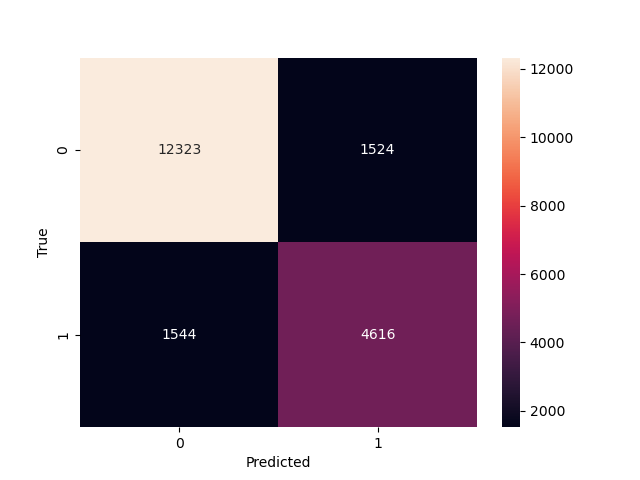
\includegraphics[width=0.75\linewidth]{images/confusion_matrix_choice}
    \caption{Enter Caption}
    \label{fig:confusion_choice}
\end{figure}

\begin{figure}
    \centering
    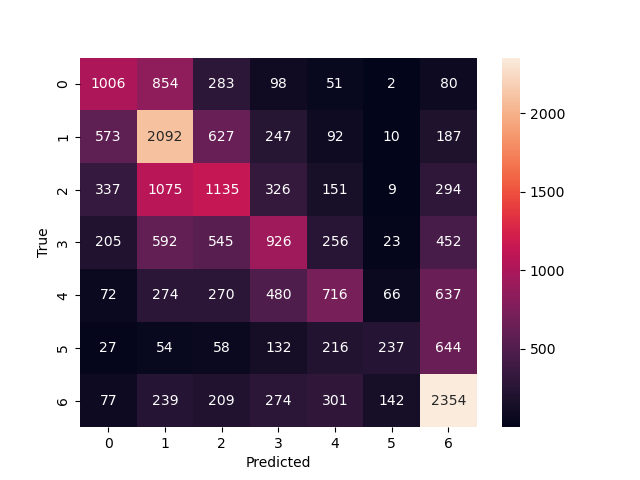
\includegraphics[width=0.75\linewidth]{images/confusion_matrix_outcome}
    \caption{Enter Caption}
    \label{fig:confusion_outcome}
\end{figure}


\begin{landscape}
\subsection{Model components}
{
\RaggedRight
\begin{table}
\small
\raggedright
\begin{tabular}{|p{5cm}|p{5cm}|p{6cm}|p{6cm}|}

\hline
\textbf{Model} &  \textbf{Type} & \textbf{Required data} & \textbf{Outputs} \\
\hline

% Decision model
\textbf{Thrombolysis decision model} 

\vspace{2mm}

Learns which patients will receive thrombolysis at each stroke team. & 

XGBoost machine learning model + SHAP model for explianability. & 

Age\newline\vspace{2pt}
Arrival-to-scan time\newline\vspace{2pt}
Onset during sleep (Y/N)\newline\vspace{2pt}
Onset time type (precise/estimated)\newline\vspace{2pt}
Onset-to-arrival time\newline\vspace{2pt}
Pre-stroke disability (mRS)\newline\vspace{2pt}
Stroke severity\newline\vspace{2pt}
Stroke team\newline\vspace{2pt}
Stroke type\newline\vspace{2pt}
Use of anticoagulants for atrial fibrillation & 

Probability of receiving thrombolysis at attended stroke team and 25 \textit{benchmark} stroke teams. \\

\hline

% Outcome model

\textbf{Stroke outcome model}

\vspace{3mm}

Learns death/disability outcome depending on patient characteristics, stroke team attended, and use/time of thrombolysis. &

XGBoost machine learning model + SHAP model for explainability. &

Age\newline\vspace{2pt}
Diagnosis of atrial fibrillation\newline\vspace{2pt}
Onset time type (precise/estimated)\newline\vspace{2pt}
Onset-to-thrombolysis time\newline\vspace{2pt}
Pre-stroke disability (mRS)\newline\vspace{2pt}
Stroke severity\newline\vspace{2pt}
Stroke team\newline &

Disability/death distribution (can be estimated with/without thrombolysis for any patient). \\

\hline

% Pathway model

\textbf{Pathway model}

\vspace{3mm}

Models flow patients through each stroke team’s thrombolysis pathway, and predicts thrombolysis use and outcomes. &

Discrete event simulation (using NumPy) array, coupled with clinical outcome model based on time to thrombolysis. &

Arrival-to-scan time\newline\vspace{2pt}
Arrive by ambulance (Y/N)\newline\vspace{2pt}
Onset known (Y/N)\newline\vspace{2pt}
Onset-to-arrival time\newline\vspace{2pt}
Scan-to-thrombolysis time\newline\vspace{2pt}
Stroke team\newline\vspace{2pt}
Stroke type &

Use of thrombolsyis and number of people mRS 0-1 under various improvement strategies:\newline\vspace{4pt}

1. Current state\newline\vspace{2pt}
2. Ascertain stroke onset times at performance of 25\textsuperscript{th} percentile stroke team\newline\vspace{2pt}
3. 30 minutes arrival-to-thrombolysis\newline\vspace{2pt}
4. Make decisions inline with \textit{benchmark} stroke teams\newline\vspace{2pt}
5. Combinations of above\newline\vspace{2pt}\\

\hline

% Pathway model

\textbf{Health economics model}

\vspace{3mm}

Estimates survival, life expectancy, QALYs, care years, and NHS care costs. &

Numerical health economics model (coded in Python). &

Age\newline\vspace{2pt}
Sex\newline\vspace{2pt}
Disability at discharge &

Survival years\newline\vspace{2pt}
Life expectancy\newline\vspace{2pt}
QALYs\newline\vspace{2pt}
Years in care\newline\vspace{2pt}
NHS care costs\\





\hline


\end{tabular}
\caption{SAMueL model components overview}
\label{tab:example}
\end{table}
}
\end{landscape}